

\chapter{Mathematical Formulation of Complex Systems}

In the last chapter, after a general theoretical section, unimolecular systems were considered in some detail. It was shown that, even for such unimolecular systems, explicit solutions for the stationary state could not be obtained, except for the hypothetical `completely linear' case. However, it was seen that the concepts of `rate-control' and `diagnostic' could give a useful insight into the workings of systems, even when there was no explicit solution. For the more complex systems, whose representation is to be considered in this chapter, the necessity of understanding a system by considering its response to parametric variation is even greater, since very little in the way of analysis can be achieved.

When the variation is differential the response of the system will be expressed naturally by a `sensitivity coefficient matrix' and in CH. III the theoretical basis of this will be developed with particular reference to how it is related to the properties of individual enzymes and how it can be estimated experimentally.

The response to finite parameter variation can only be studied by means of numerical experiments performed on mathematical models. In CH. IV a computer system capable of flexibly performing such `in numero' experiments on a variety of general systems is discussed.

The contents of this chapter will, then, be concerned with the problem of formulating complex metabolic systems. in the mathematical terms suitable to computer analysis. After discussing the distribution between a `subsystem' and a `complete' system and initially restricting consideration to subsystems, the network of genial reactions is introduced.

This lifts the previous restriction to unimolecular reactions and in addition allows the representation, via suitably complex rate expressions, of `allosteric' enzymes, where substances can influence the rates of reactions from which they are metabolically remote. Next it will be shown that, for systems where it is wished to consider the effects of substituting alternative alleles for structural genes, a new type of genotypic parameter can be introduced by extending the idea of a `rate expression'. The section ends by considering how the effects of 'growth' and 'enzyme regulation' may be represented for subsystems.

Finally an approach is made to the problem of formulating `complete systems', which gives consideration to the allocation of resources by differential gene activity.

\section{Subsystem and complete system}

An dynamical system of the type which was discussed in CH.I (1.1) involves the assumption that some metabolites, denoted by $S_{1}, S_{2} \cdots,$ are \underline{within} the system and are variables, whereas others $X_{1}, X_{2} \cdots$, are \underline{outside} the system and have the status of parameters. The assignment of any metabolite to one of these two classes is clearly a quantitative judgement and has up till now been made on the reasonable basis that the medium had a relatively large volume and approximated to an infinite source or sink, thus rendering the concentration environmental metabolites almost constant. However the assignment is clearly arbitrary and cannot de applied in certain situations, where it becomes necessary to widen the system so as to include at least some `environmental metabolites as variables, for example if it is wished to consider `growth in a chemostat.

Even when the environmental metabolic boundary can be accepted a difficult problem arises because of the necessity of reducing the large number, many thousands, of metabolites which are involved in a `real' system. One way in which this reduction can be performed, for our stationary state studies, is by eliminating system variables which are not directly of interest, a technique which has already been used to eliminate unwanted enzymic intermediates. However, this was possible only because, on the assumption that protein-protein interaction was negligible, the necessary eliminations involved only linear equations in the enzymic intermediates and were already fully treated under the subject of steady state enzyme kinetics. The equivalent technique at the level of intermediary metabolites is not in general possible because non-linear equations are involved. For example it might involve eliminating metabolites within a sequence of enzymes and replacing the sequence by a single `enzyme' with a complex rate expression, a task which, as was seen in CH I, has no explicit algebraic solution. Hence, in general, no such exact reduction can be made. It may, however, prove possible to find closed algebraic expressions which are a reasonably good description of pathway behaviour, provided that the remaining system variables lie within certain ranges.

In these circumstances it is necessary to view the problem of reduction in a flexible way; 'what is a reasonable reduction in one situation may be quite unreasonable in another. One extreme is the situation when the parameter changes being studied are likely to have large effects throughout the whole metabolic system, even though the varied parameters may themselves all be within one pathway. Changes which, for example, markedly affected growth rate would seem to be of this type. In this case there is no escape from considering some representation of the `complete' system . The representation being, perhaps, detailed only in the region of the parameter changes, it being sufficient elsewhere to represent the functioning of whole areas of metabolism, as for example the glycolytic pathway, in some approximate way. Some consideration will be given to the rather difficult problem of such complete systems at the end of this chapter.

Another way in which the desired reduction can be made is to consider the area of metabolism in which parameter variation is to be made as a `sub-system'. This involves arguing that internal metabolites which are `remote' from the sub-system will remain more or less constant and can be formally treated as `external' metabolites.

The criteria for deciding what constitutes such a sub-system are not simple. The correct decision is clearly a quantitative matter and will depend, inter alia, on the size of the parameter variations. In general, the larger the variation the larger will have to be the sub-system. Despite the difficulty in defining exactly what is meant by a subsystem, in this sense, there is no alternative but to use the concept.

\section{Network of general enzymically catalysed transformations}

Until now we have considered systems of effectively unimolecular reactions, where the transformations, taking place within a fixed volume, are represented in a system diagram by steps of the type:

\centerline{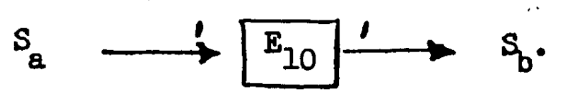
\includegraphics[scale=1]{figure2_pathway10.png}}

This means that the 10th enzyme catalyses a unimolecular conversion from $S_{a}$ to $S_{b}$ in the sense that for every molecule of $S_{a}$ removed one of $S_{b}$ is produced. The net-flux/unit quantity of enzyme, taken as +ve in the arrowed direction, was given by a rate-expression which assumes enzymic intermediates to be at a stationary state with respect to $S_{a}$ and $S_{b}$ and which takes fully into account that the reaction $S_{a} \longrightarrow S_{b}$ can be reversible.

This can easily be generalised to allow for enzymically catalysed reactions of arbitrary complexity. For example the reaction
%
\begin{equation}
S_a + S_b \rightleftarrows S_c + 2 S_d
\label{eqn:21}
\end{equation}
%
is symbolised by

\centerline{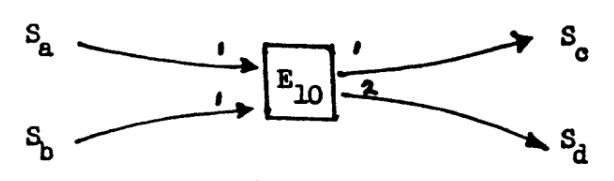
\includegraphics[scale=0.65]{figure2_E10.png}}

and has a rate-expression/unit quantity of enzyme giving the net flux towards, say, the metabolite $S_{c}$ of $f_{10}\left(S_{a}, S_{b}, S_{c}, S_{d}, \ldots.\right)$. Clearly the corresponding rate expressions for the metabolites $S_{a}, S_{b}, S_{d}$ are $-f_{10},-f_{10}$, and $+2 f_{10}$ respectively where the appropriate stoichiometric constants $-1,-1,2$ are obtained from the equation (2.1) for the net reaction. The symbol $f_{10}$ stands here for either the function or its value, depending on the context.

In a general network of reactions, if $f_j$ is the rate expression for unit quantity of the jth enzyme referred to one of its products, then $\lambda_{ij} f_j$ will be the appropriate rate expression of the $j$th enzyme for the ith metabolite.

The \underline{`stoichiometric matrix'} $\left[\lambda_{ij}\right]$ will consist of small integers, mostly 1 and $-1$, and zeros and will in fact contain mostly zeros, since most enzymes remove or produce only a few metabolites. In a system having $n$ metabolites and $m$ enzymes $\left[\lambda_{i j}\right]$ will be an $n \times m$ matrix.

The figure below represents a general system existing in a given volume $V$ and with total quantity, $\mathrm{E}_j^T$ of the jth enzyme. This can be distributed in any way throughout the volume or, if a transport enzyme, upon the surface.

\centerline{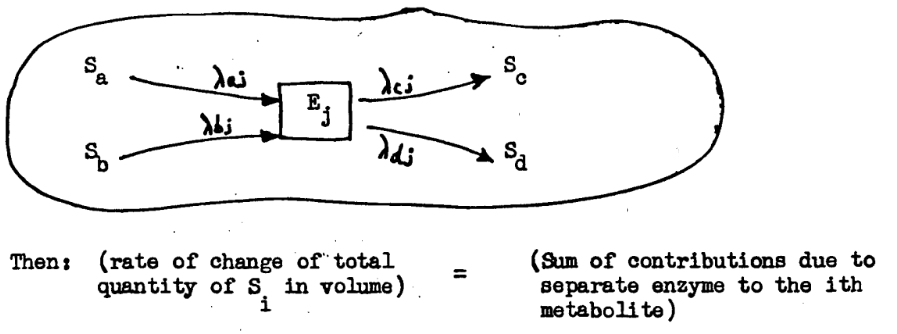
\includegraphics[scale=0.8]{figure2_1.png}}

%Thenr (rate of change of total $=$ (sum of contributions due to quantity of $S_{i}$ in volume). separate enzyme to the ith metabolite)

\begin{figure}
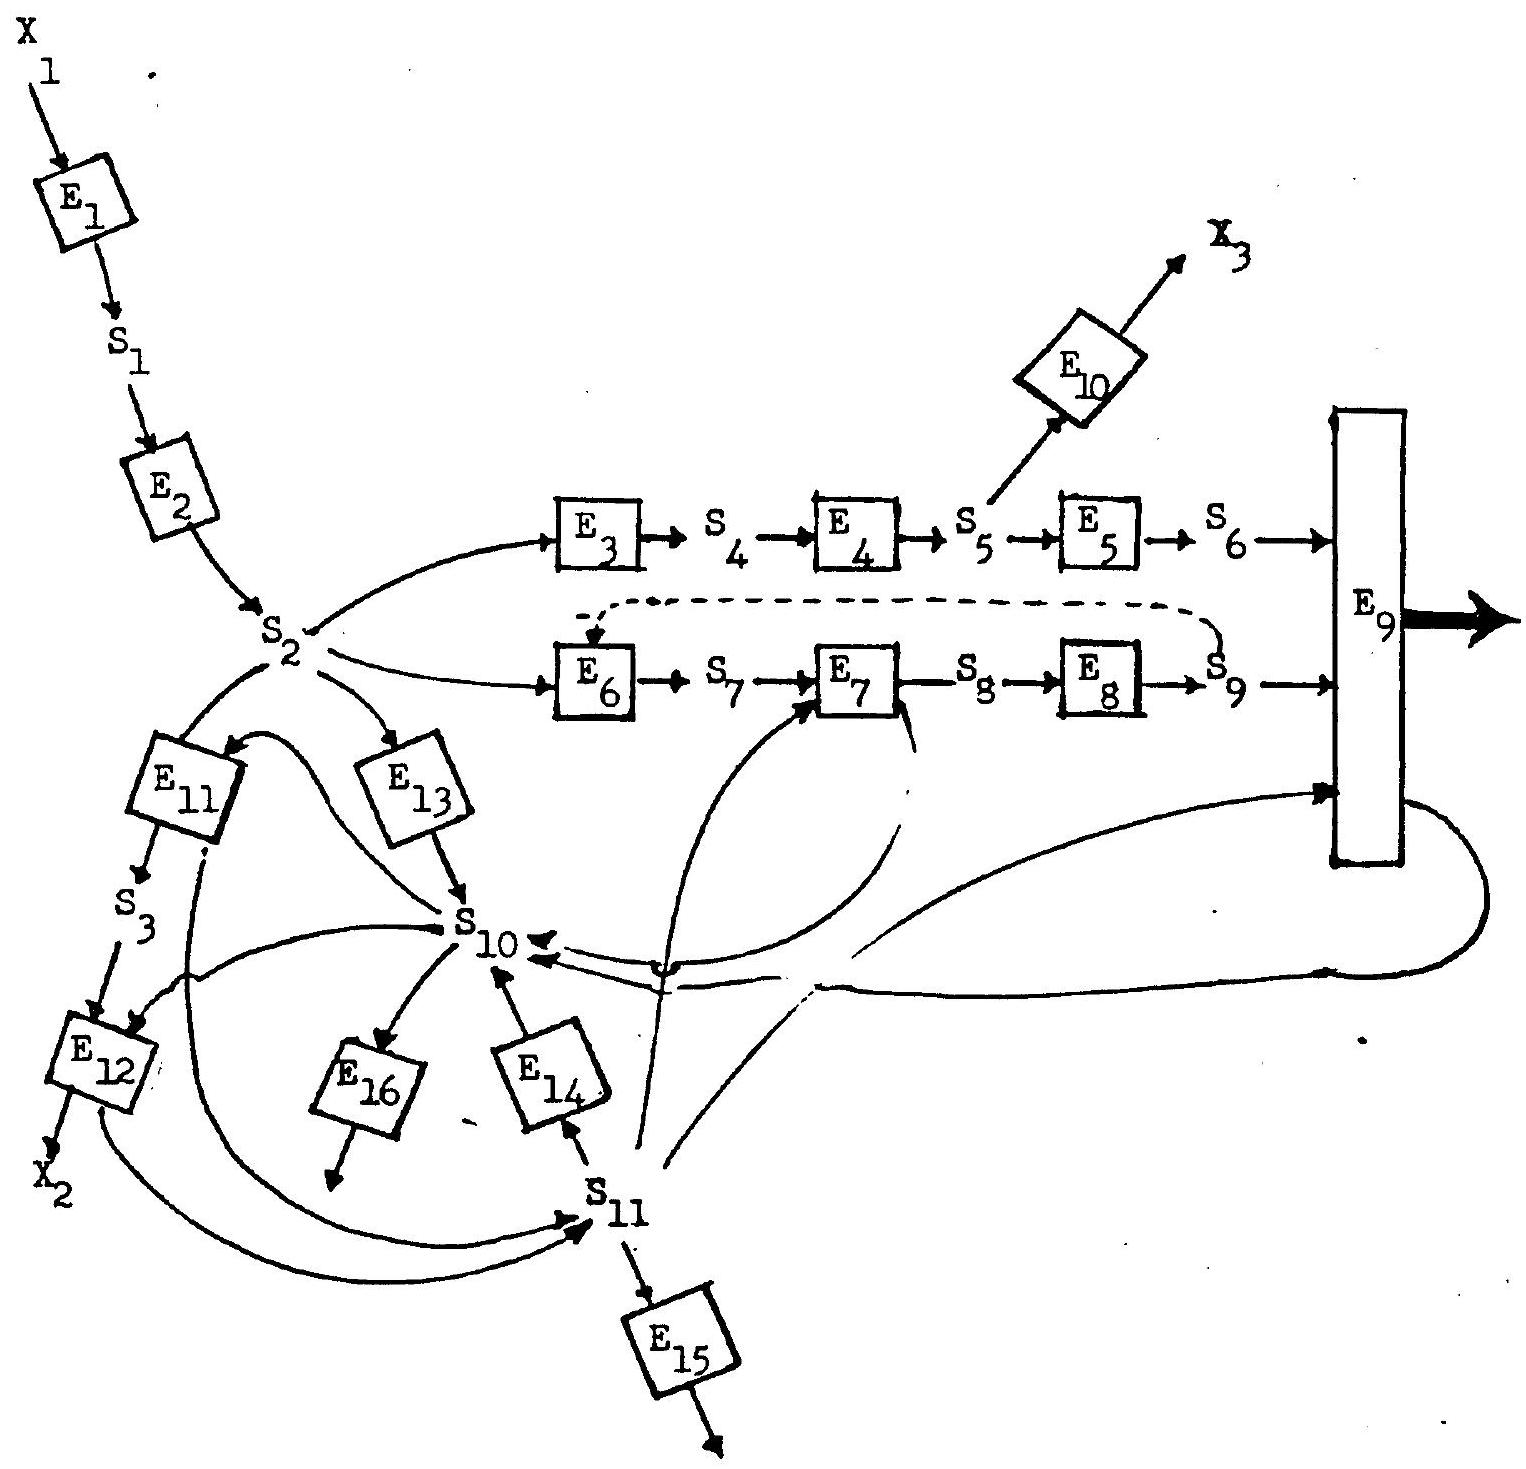
\includegraphics[scale=0.2]{2023_01_30_a974a42f7b7381f3f940g-068}
\caption{METABOLIC STRUCTURE}
\end{figure}

\begin{figure}
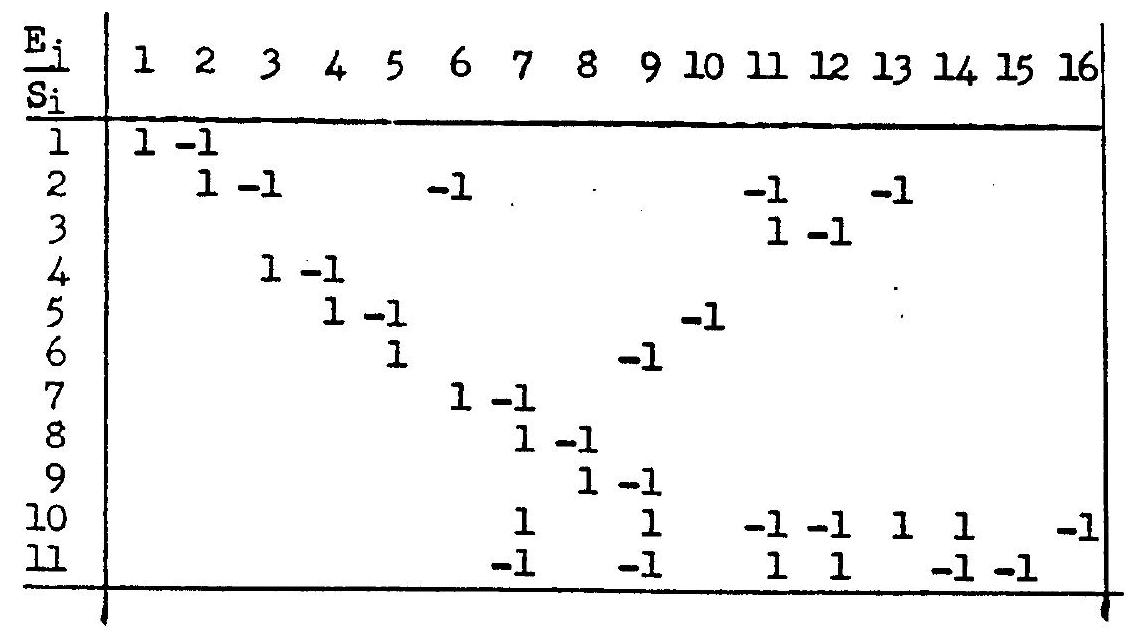
\includegraphics[scale=0.25]{2023_01_30_a974a42f7b7381f3f940g-068(1)}
\caption{STOICHIOMETRIC MATRIX}
\end{figure}

\begin{equation}
\frac{d (S_i \times V)}{dt} = \sum_j \lambda_{ij} E_{j}^{T} f_{j}(\ldots)
\label{eqn:22}
\end{equation}
%
or
%
$$
\dot{S_i} =\quad \sum \lambda_{i j}\left(\frac{E_{i}^T}{V}\right) \cdot f_{j} - \left(\frac{1}{V} \dot{V}\right) \cdot \dot{S}_{i}
$$
%
Writing $\frac{E_{j}^{T}}{V}=E_{j}$ the effective concentration of the jth enzyme in the system and remembering that  ($1/V \dot{V})=0$ we have the dynamical functions $\varphi_{i}$ for the general system as
%
\begin{equation}
\varphi_{i}=\dot{S}_{i}= \sum \lambda_{i j} E_{j} f_{j}(\ldots)= \sum \lambda_{ij} F_{j}
\label{eqn:23}
\end{equation}
%
In (2.3) $\mathrm{F}_{\mathrm{j}}$ is the net flux carried by the $\mathrm{jth}$ enzyme in unit volume of the system, the flux being defined by reference to one of the substrates of the $j$th enzyme.

The general equation (2.3) will be made more concrete by means of an example, shown in fig (1), which will illustrate how various metabolic situations can be represented. This example will also be used to discuss certain conditions to which the equations (2.3) must conform.

The metabolic network of fig (1) comprises 16 enzymes, 10 intermediate metabolites and four external substances and the general meaning of the metabolic scheme is as follows. $X_{1}$, which can be regarded as a nutrient, is transported in an converted to $S_{2}$ at which point the metabolism divides into several pathways. A catabolic pathway, $S_{2} \rightarrow S_{3} \rightarrow X_2$, yields a high energy product $S_{11}$ by bimolecular coupling reactions at steps 11 and 12. Two biosynthetic pathways, $\mathrm{S}_{2} \rightarrow \mathrm{S}_{4} \rightarrow \mathrm{S}_{5} \rightarrow \mathrm{S}_{6}$ and $\mathrm{S}_{2} \rightarrow \mathrm{S}_{7} \rightarrow \mathrm{S}_{8} \rightarrow \mathrm{S}_{9}$ converge onto a condensing reaction at step 9, the second of these pathways and the condensing reaction being coupled to the high energy product $\mathrm{S}_{11^{*}}$

Clearly $S_{10}$ and $S_{11}$ have a similar role to that of ADP and ATP in a real system and the step $\mathrm{E} 9$ would correspond to protein synthesis. Continuous lines represent a net flux of metabolite, whilst the arrow and the number above it indicate the algebraically positive direction and stoichiometric constant respectively. Dotted lines indicate metabolites influencing the rate of a reaction, without themselves being appreciably consumed, the sign above the arrow indicating, when appropriate, whether there is an inhibitory or excitatory effect. Thus in the figure it can be seen that $S_{9}$ exerts feedback inhibition on $E 6$ the last enzyme in its own pathway, or again the external substance $X_{4}$ activates the last enzyme in the same pathway. All these effects are taken fully into account by multiplying the stoichiometric matrix $\lambda_{i j}$, shown below the figure, into the set of rate expressions, $f_{1}, \cdots, f_{16}$ to produce the 10 functions $\varphi_{1}, \cdots, \varphi_{10}$ The dynamical functions can then be used, as explained earlier, to obtain the stationary solution and the sensitivity of any measures to any parameters which are of interest. Thus the problem of describing the system mathematically is just that of writing dorm the set of rate expressions, $f$. How exactly this is done will depend on what qualities are considered to be possessed by the separate enzymes. For instance the unimolecular expressions $f_{1}, f_{2}$ may simply be of the usual linear form (1.13b) unless it is suspected that their saturation properties are important. Other expressions clearly have to be more complex just to represent the effects encoded in the metabolic diagram. For example, the simplest possible rate-expression for the bimolecular reaction of $\mathrm{E}_{11}$ would be
%
$$
f_{11}(\ldots .)=k_{x}\left(S_{2} \times S_{10} - S_{3} \times S_{11} /K_{10}\right)
$$
%
and this, of course, takes no account of saturation effects. Again there are various possibilities for representing $\mathrm{E} 6$, which is sensitive to feedback inhibition from $S_{9}$, one of the simplest being
%
$$
f_{6}(\ldots)=k_{1 x}\left(S_{2} - \frac{S_{7}}{K_{6}}\right) \times \frac{1}{\left(k_{2} + S_{9}\right)}
$$
%
The situation then is that metabolic `structure' of considerable detail can be included in the functions $\varphi_{1}, \cdots, \varphi_{10}$ by means of the matrix $\left[\lambda_{i j}\right]$ and the set of rate-expressions. In general these rate expressions should be of the simplest form which will express the desired properties of the separate enzymes, However, the general set of equation $(2.3)$ must satisfy a certain condition as will be discussed in the next section.

\section{Necessity for linear independence of the functions}

This arises because if it happens that one of the $\varphi_i$ is simply a linear combination of others there will not be sufficient simultaneous equations to determine the stationary solution. Since the rate expressions are clearly all independent functions this condition of linear independence is just that the rows of $\left[\lambda_{ij}\right]$ be linearly independent.

An example will show how faulty formulation of a set of equations may generate dependence. In formulating a system involving, say, a set of ADP/ATP dependent reactions, it might be thought sufficient to link the generating system to the absorbing system by a closed loop. In terms of our model fig (1) this is equivalent to omitting the steps E13 (generation ADP), E15 (degrading ATP) E16 (degrading ADP). This might appear to satisfy the linked steps E11 and E12.

The rates of change of the two substrates, $S_{10}$ and $S_{11}$ would then be:
%
$$
\begin{aligned}
\dot{S}_{10} &= \varphi_{10}=-F_{11}-F_{12}+F_7+F_9+F_{14} \\
\dot{S}_{11} &= \varphi_{11}=+F_{11}+F_{12} - F_7-F_9-F_{14}
\end{aligned}
$$
%
For the stationary state conditions we find that $\varphi_{10}=0$, implies that $\varphi_{11}$ is determined also to be zero and imposes no separate condition. This eliminates one of the $n$ necessary equations for solution. Dynamically the system would have the property $\frac{d\left(S_{10}+S_{11}\right)}{dt}=0$ so that the sum of ATP and ADP could not change and would be dependent on the initial conditions (viz, the initial value of the sum). In addition the matrix $D=\left[\frac{\partial \varphi_{i}}{\partial S_{j}}\right]$ would have no inverse thus invalidating the iterative method of (1.9). A biochemical system formulated in this way would thus not have the property that the stationary state was dependent only on genetic and environmental parameters, and the whole theoretical approach outlined earlier would be invalid.

It seems reasonable to argue that this difficulty arises out of the unreality of formulating a system in which production of ATP is always coupled to removal of ADP and vice versa. The solution of the difficulty then is to extend the system by adding the reactions E13, E15, E16, which allow $\mathrm{S}_{10}$ and $\mathrm{S}_{11}$ to participate in non-coupled reactions and thus renders $\varphi_{10}$ and $\varphi_{11}$ linearly independent.

It may be objected that the investigator wishes to consider a situation where the sum of ATP and ADP is at a previously prescribed level. This is of course still possible with the extended model. The difference being that instead of the sum being determined by initial conditions it must now be determined by parameter values acting within the system. For example, suppose the reaction El3 is an irreversible reaction saturated by $S_{2}$ and providing a flux/ unit volume determined by a parameter $k_{1}$ and that E16 and E15 are linear and irreversible with the same effective rate constants $k_{2}$ Then at S.S.,
%
$$
\varphi_{10}=-F_{11}-F_{12}+F_{7}+F_{9}+F_{14}+k_{1}-\left(k_{2} \times \olsi{S}_{10}\right) = 0
$$
%
and $\varphi_{11} = -\mathrm{F}_{11}-\mathrm{F}_{12}+\mathrm{F}_{7}+\mathrm{F}_{9}+\mathrm{F}_{14}+\mathrm{k}_{1}-\left(\mathrm{k}_{2} \times \olsi{\mathrm{S}}_{11}\right)=0$ so that
%
$$
\left(\olsi{S}_{10} + \olsi{S}_{11}\right) = k_{1}/k_{2}
$$
%
Therefore by adjusting the parameter $k_{1}$ the investigator can prescribe the sum of ATP and ADP.

In general then only systems, having the property that the rows of $\left[\lambda_{ij}\right]$ be linearly independent, will be considered, additional reactions being added if the condition is not at first satisfied. This will ensure the applicability of the mathematical methods outlined earlier for calculating the sensitivity coefficients whilst not restricting the investigator in any important way.

\section{Independent fluxes in a system}

An important `measure' in a system is often the stationary flux/unit vol, $\olsi{F}_{j}$, at some step in the network, there being $m$ such measures in a system having $m$ enzymes. However, these stationary fluxes are not independent since there are $n$ conditions connecting them, namely
%
\begin{equation}
\varphi_{i}=\sum \lambda_{i j} \olsi{F}_{j}=0 \mbox{ For } i=1 \mbox{ to } n
\label{eqn:24}
\end{equation}
%
The number of independent fluxes will thus be the number of enzymes less the number of conditions connecting them or $(m-n)$.

For example, in a straight chain the number of enzymes will only be one more than the number of pools and hence there is just one independent or `pathway' flux.

For the more complex system of fig (1) there are 16 enzymes and 11 pools so that there are 5 independent fluxes. This means that if 5 selected fluxes are known the remaining 17 can be found using the condition (2.4). This amounts to inverting part of the matrix and may appear algebraically complex. However, the connection between the fluxes can be seen immediately from a metabolic diagram. Thus, if the 5 excretory fluxes $F_{0}, F_{10}, F_{12}, F_{15}, F_{16}$, in fig(1) are selected as metabolically significant the other fluxes can be written down in terms of them as for example:
%
\begin{equation}
\begin{aligned}
& \olsi{F}_5=\olsi{F}_9 \\
& \olsi{F}_4=\olsi{F}_9 + \olsi{F}_{10} \\
& \olsi{F}_6=\bar{F}_9 \\
& \olsi{F}_{11}=\olsi{F}_{12} \\
& \olsi{F}_{13}=\olsi{F}_{16} + \olsi{F}_{15} \\
& \olsi{F}_2=2 \olsi{F}_9 + \olsi{F}_{10}+\olsi{F}_{12}+\olsi{F}_{16}+\olsi{F}_{15}
\end{aligned}
\label{eqn:25}
\end{equation}
%
For most metabolic systems the number of enzymes will only slightly exceed the number of metabolites so that in fact there are relatively few independent fluxes in a network.

\section{Introduction of genotypic parameters}

Suppose that in the 16 enzyme system of fig. (1) alternative enzymes were available at various steps in the network, then the particular set of enzymes possessed by such a 16 enzyme `organism' would depend on its set of alleles or its `genotype'. The introduction of a set of ``genotypic parameters'' ( $\pi_{1}, \pi_{2}, \cdots, \pi_{16}$ ) specifying. the allelic situation at each step. will serve to describe the genotype. For example in a haploid organism with two alleles at each locus the $\pi$ integers must each take one of two values, whereas if the organism were diploid there would be three possible values since at each locus there are, physiologically, three alternative states, Figure (2), homozygous either way and heterozygous.

\centerline{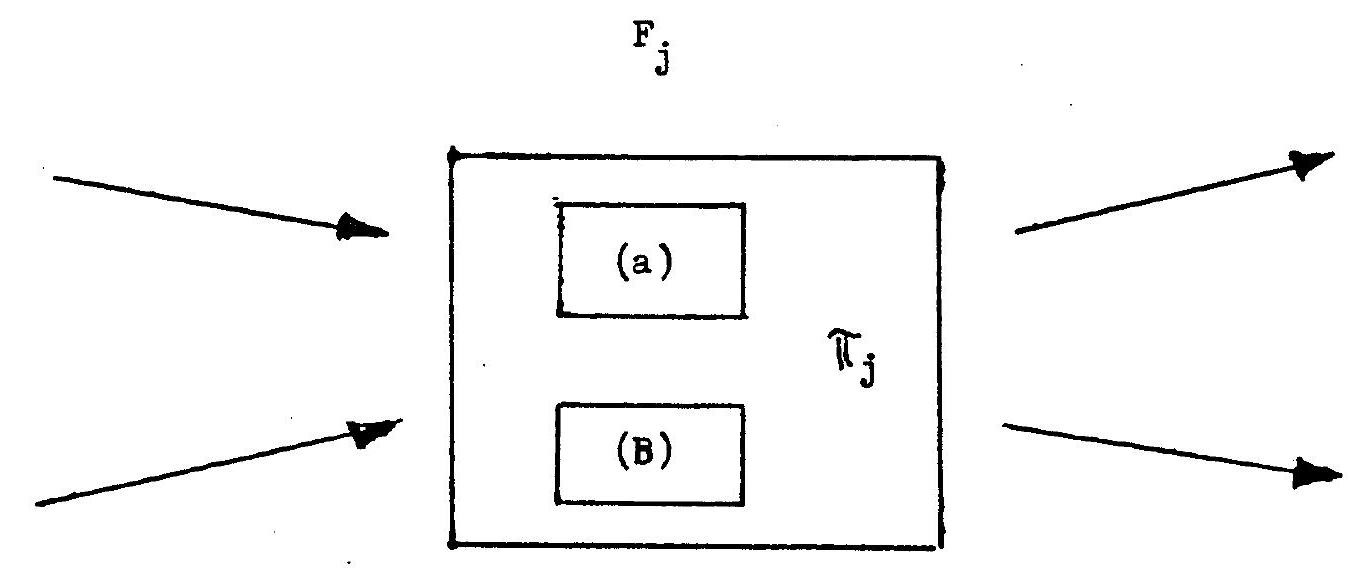
\includegraphics[scale=0.5]{2023_01_30_a974a42f7b7381f3f940g-076}}

The flux depends on the allelic enzymes $E_{j}^{a}$ and/or $E_{j}^{b}$. The $\pi$ value specifies the allelic state of the locus.

\begin{figure}
\centering
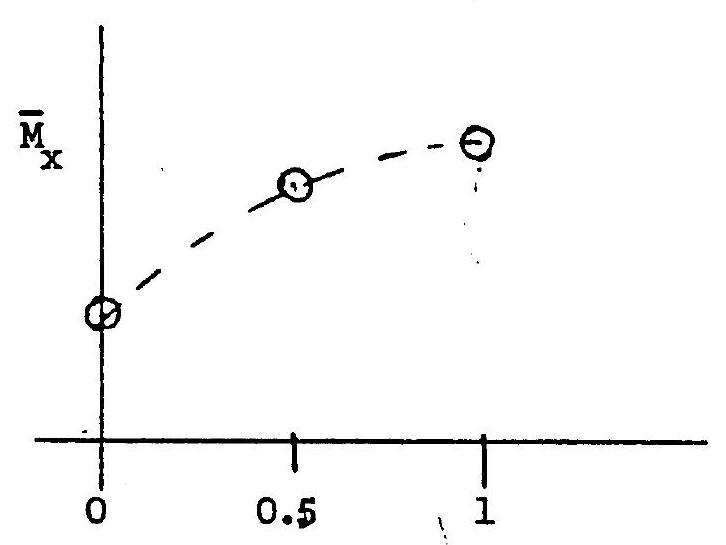
\includegraphics[scale=0.26]{2023_01_30_a974a42f7b7381f3f940g-076(1)}
\caption{The measure $\olsi{M}_{x}$ as a function of the value of $\pi$.}
\end{figure}

Consideration of the phenotype/genotype, or Ph/Ge relation will clearly be facilitated if these ir parameters can be included in the specification of the functions $\varphi_1 \cdots, \varphi_{n}$. This can conveniently be done by extending the idea of a rate expression, the new formulation depending on the ploidy and the number of alternative alleles at each locus. The case of two alternative alleles per variable locus will be considered for haploid and diploid organisms.

Thus for a haploid organism suppose that the alleles for the jth locus give alternative enzyme concentrations $\mathrm{E}_{j}^{\mathrm{a}}$ and $\mathrm{E}_{j}^{\mathrm{b}}$ and alternative rate expressions $f_{j}^{a}(\ldots)$ and $f_{j}^{b}(\ldots$) , it being noted that these expressions may be of quite different form as for example one being sensitive to end product inhibition and the other not. A composite expression (cf. Fig. (2)) can be written for the flux/unit volume at the jth step thus.
%
\begin{equation}
F_{j}=\left(1-\pi_{j}\right) E_{j}^{a} f_{j}^{a}(\cdots)+\pi_{j} E_{j}^{b} f_{j}^{b}(\cdots)
\label{eqn:26}
\end{equation}
%
and clearly $\pi_j = 0$ gives the (a) allele and $\pi_i = 1$ gives the (b) allele so that 0 and 1 are the possible values for $\pi^{j}$

Since the description is formally the same as before, only with a more complex set of rate expressions which involve the if $g$ the same numerical techniques will work. In particular it will be possible to consider how a measure $\olsi{X}$ depends on the set of alleles constituting the genotype since the non algebraic functional relationship
%
\begin{equation}
\olsi{M}_{X}=\olsi{M}_{X}\left(\pi_{1}, \pi_{2}, \ldots, \pi_{16}\right)
\label{eqn:27}
\end{equation}
%
can now be investigated numerically.

For a diploid organism it is only. necessary to allow the $h_{j}$ to take three values, $0,1/2,1$, where $\pi_{j}=1/2$ corresponds to the heterozygous state at the $j$th locus. This involves the assumption that enzyme quantity is proportional to gene dosage which seems reasonable so long as enzyme quantity is till treated as a genetically specified parameter. The response of a measure to $\pi_{j}$ indicated in fig. (2) now gives an indication of the importance and the degree of dominance of the $j$th locus and the effect on this of varying other $\pi_{j}$, that is the genetic background, can be tried.

The introduction of the or notation makes clearer what is meant by the Ph/Ge relation. It also reveals a difficulty not previously raised. Thus the_Ph/Ge response matrix $\left[\mathrm{C}_{\mathrm{P}_y}^{\mathrm{M_X}}\right]$ of (1.9) can now be recognised as $[C^{\olsi{M}_X}_{\pi_y}]$ but since ${\pi}_y$ can only assume discrete values the meaning and usefulness of the differential sensitivity analysis will have to be considered. The uses of the general relationship (2.7) in the framework of theoretical ! population genetics will be discussed in CH.V.

\section{Non-enzymic transformations}

In metabolism there will be many situations where non-enzymic transformations are important, e.g. in the case of surface transport by simple diffusion. These can be represented perfectly well using rate expressions the only difference being that instead of enzyme concentration there will be some other factor. Thus `non-enzymic transport' rate-expressions will involve the quantity area/volume, or $A/V$. That is the 'concentration of area' rather than the concentration of enzyme. Enzymically mediated transport expressions will not involve $A/V$ since the amount of surface over which the enzyme is distributed is not relevant. The inclusion of nonenzymic transformations will not alter the general form of (2.8) except that a new category of pseudo-enzymes are introduced.

\section{Expanding systems}

It is often of interest to consider growing systems, particularly since the condition of steady or exponential growth of a culture of such systems is a well defined experimental situation: such a growing system clearly does not possess a stationary state, since certain system parameters are no longer constant with time.(Grainger, 1966, 1968).

However, subject to the conditions that these parameters do not vary too rapidly or over too wide a range and that the system itself is intrinsically stable (see next section) the stationary state approach still proves useful.

Thus an investigator of such a non-stationary system would be interested in the mean values over time, $\left\langle S_{i}\right\rangle_{t_1}$ of system variables. Given the above conditions the $\left\langle S_{i}\right\rangle_{t}$ will be well approximated by the stationary $\olsi{S}_{i}$ corresponding to average values of varying parameters. In fact fluctuating parameters in a growling system are often quite well behaved In the above sense. For example in a spherical cell which continuously doubles its volume and then divides, perhaps representing a growing bacterium, the parameter (A/V) suffers a sharp increase of $\approx 25 \%$ at each division and then gradually falls to reach its former value just prior to the next division. Thus, given reasonable metabolic stability, the system will be close to a stationary solution during most of the time and will suffer its greatest disturbance at each cell division. A similar situation holds for the parameter combinations 'relative gene dosage', whose importance will be seen in the section on control. These double at certain points in the cell cycle when each gene is duplicated and decline steadily during the rest of the cycle due to other genes being replicated. For syncytial growth the stationary state assumption may be a very good approximation, thus (A/V) will vary hardly at all during the tube like growth of hyphae and the `relative gene dosage' will remain almost constant since in this case a number of asynchronously dividing nuclei inhabit a common metabolic space. Supposing then that it is acceptable to study the stationary state corresponding to average parameter values the effect of growth on this S.S. will still have to be allowed for. This arises because it is no longer permissable to assume $\dot{V}=0$ when simplifying the dynamic equations (2.2). Thus instead of the form (2.3) there arises

\begin{equation}
\varphi_{i}=\dot{S}_{i}=\sum \lambda_{ij} E_{j} f_{j}(\ldots)-(1/V \dot{V}) \cdot S_{i}
\label{eqn:28}
\end{equation}

Clearly a stationary. solution with growth will require all $S_{i}$ constant and $\dot{V} \neq 0$ and will only be possible if the term $(1/V \dot{V})$ is constant. This means that such growth will be exponential with growth constant $G$, where
%
$$
G = \frac{1}{V} \dot{V}
$$
%
Since, for the present, only `subsystems' are being considered $G$ has to be treated as a parameter. The equations (2.8) are then formally equivalent to a metabolic system within a fixed volume and having a ``flux to expansion'' of $G \times S_{i}$ away from each $S_{i}$. Whether these expansion terms will constitute more than a minor correction will depend on the metabolic pathways contained in the subsystem. In any particular case the G constant will, of course, be known and the problem in setting up the model is to assign levels to the $E_{j}$ consistent with general data.

For example in the arginine pathway it may be known that arginine in pool form is of the order of $5 \%$ of arginine in protein in which case the ${E}_{j}$ in arginine pathway would be adjusted until the terms $\lambda_{i j} E_{j} f_{j}(\ldots)$ are approximately twenty-fold greater than GS$_{\text {arg }}$. This involves some guesswork but can usually be done satisfactorily. The expansion terms can usually be ignored in major pathways such as the glycolytic, which carry a large flux, but may be of dominant importance in pathways carrying a small flux such as co-enzyme synthesis. In addition any mutants tending to block the flux in a pathway and at the same time raise the pool levels will enhance the importance of the expansion terms.

\section{Stability of networks of general reactions}

The unimolecular systems studies previous were fairly generally $\gamma$ stable. The more general reactions now under discussion do not, (Higgins, 1968), possess any general, stability property but there is nevertheless reason to suppose that stability may be a common property. This is suspected because in a large system it will often be the case that the dynamics of a part of it, for example a single pathway, will approximate to that of a pseudo-unimolecular system which is known to be stable. However, since the interaction of stable sub-systems can produce large scale instability no general assertion can be made. Further evidence of a tendency to stability is that the dynamical matrix $[\mathrm{D}]$ will almost invariably have all its diagonal elements -ve.

\section{Control by repression and induction of gene activity}

{\bf Control of enzyme quantity by repression and induction of gene activity}

This phenomenon, which is widespread can be expected to be important in determining the response of a system to its environment. Subject to certain restrictions it can be represented fairly adequately and involves the addition of a `control level' to the type of system previously discussed. Thus in the example given in fig. (1), which had 16 structural genes and directly specified not only the rate expressions but also the enzyme concentrations there would be added a set of regulator genes. The regulator genes are assumed to produce very small concentrations of control proteins on a more or less constitutive basis. Some of the structural genes then have their activity controlled either separately or in groups by these control proteins which can be thought of as 'transducers' able to receive signals from concentrations of specific intermediate metabolites. This can be represented diagrammatically by extending the genetic level of fig. (1), as indicated below.

\begin{center}
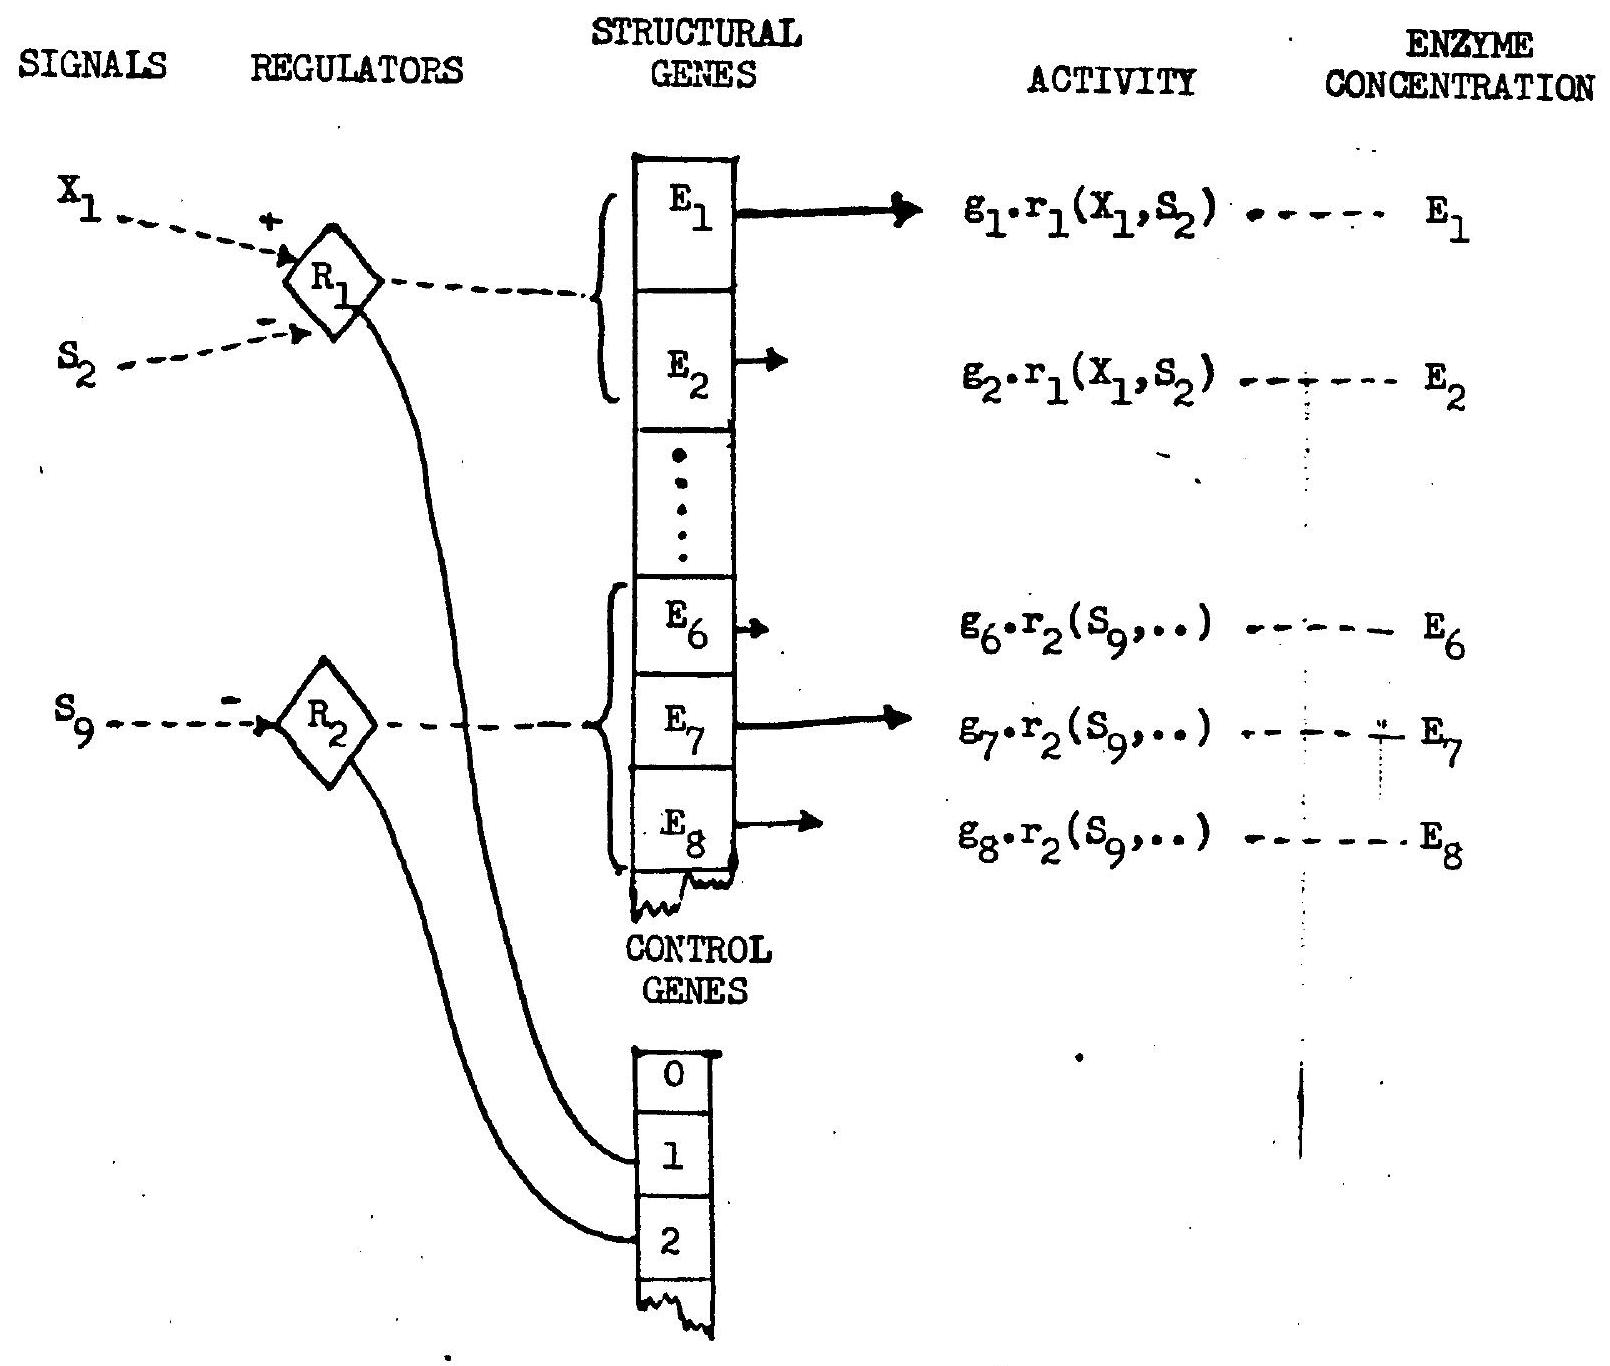
\includegraphics[max width=\textwidth]{2023_01_30_a974a42f7b7381f3f940g-083}
\end{center}

Thus the regulatory protein, represented functionally by say a block of type {(\color{red}Diamond R)} has a `regulatory function', $r_1 (X_1, S_2)$, representing induction by $\mathrm{X}_{1}$ and endogenous repression by $\mathrm{S}_{2}$ and this acts co-ordinately on the enzymes $\mathrm{E}_{1}, \mathrm{E}_{2}$ of the initial pathway. Or again the three enzymes E6, E7, E8 are coordinately repressed by the end product of their pathway, $S_{9}$. Enzymes not subject to control can be formally thought of as under, the control of $R_{0}$ which produces constant gene activity The constants $g_{1}, g_{2}, \ldots$ are determined by the structural genes for enzymes $E_{1}, E_{2}, \ldots$ and are a measure of their intrinsic messenger producing power, thus if two copies of the same structural gene were present its `g' constant would be doubled. The regulatory functions $r_{1}(\ldots)$.. etc. will be represented by suitable algebraic expressions. with values lying between `1' and `0' representing maximum and zero gene activity respectively. Unlike `rate-expressions' there is little theoretical basis for such functions and they are intended only to represent what is known or surmised about the functional aspects of regulation. For example the feedback from $S_{9}$ mediated by the function $r_{2}$ may be of the form $r_{2}\left(S_{9}\right)=1 /\left(1+S_9\right)$, the gene having half of maximal activity at unit concentration of $S_{9}$. More complex functions can express the known features of regulation somewhat better and this will be returned to in $\mathrm{CH}$ IV.

The relation of enzyme concentration to gene activity involves making a number of rather general assumptions and in addition cannot be discussed without involving a `complete' system. However, for the case of a subsystem which can be regarded as a small part of a larger system then the level of an enzyme in the subsystem will be proportional to the activity of its structural gene. Subject then to this restriction that the subsystem is a small part of the whole of metabolism, it becomes possible to consider control loops acting within the subsystem and also from its 'environment', which now includes `constant' internal metabolites, by extending the general equation (2.3) to be
%
\begin{equation}
\varphi_{i}=\sum \lambda_{ij} g_{j} f_{j}(\ldots) \cdot \eta_{jk} {r_{K}}(\ldots)
\label{eqn:29}
\end{equation}
%
Here summation is over $j$ and $k$ and $[\eta{jk}]$ is a regulatory matrix showing which regulator genes control which enzymes. Even when such `control' is added the mathematical situation is unchanged except that an additional type of `block' has to be considered in arriving at the $\varphi_{i}(\ldots$) . The formulation of a system now consists in providing all rate expressions and all regulatory functions together with the stoichiometric and regulatory matrices $\lambda_{ij}$ and $\eta_{jk}$

The introduction of `genotypic parameters', via relation \eqref{eqn:26} , previously assumed, in the diploid case, that enzyme concentration was proportional to gene dosage. If genotypic parameters are embedded in a system with a `control' level this becomes the much more reasonable assumption that 'capacity' for gene action, or the value of g, constants,  is proportional to dosage. If it is further assumed that the alternative alleles at a locus are regulated in parallel, which will often be the case, then (2.9) becomes
%
\begin{equation}
\varphi_{i}(\ldots)=\sum_{j, k} \lambda_{ij}\left[\left(1-\pi_{j}\right) g_{j}^{a} f_{j}^{a}(\cdots)+\pi_{j} g_{j}^{b} f_{j}^{b}(\ldots)\right] \eta_{j  r_{k}}(\ldots)
\label{eqn:210}
\end{equation}
%
\section{Complete growing systems}

On p.58 we considered how to formulate a subsystem within a steadily growing larger system. The effect of growth on pools and fluxes within the subsystem was allowed for by adding an extra flux to expansion' term, $G \times S_i$ away from each pool when formulating the equations for the S.S. The exponential growth constant, $\left.G=\left(\frac{1}{V}\right) {\dot{V}}\right)$, was, in these circumstances, assumed to be given as a fixed parameter. Clearly this is not an adequate formulation if we wish to consider problems such as how the growth constant $G$ itself arises as a system measure and how it is dependant, via the complete system, on the various genetically specified parameters.

The problem of formulating the necessary `complete' systems is theoretically rather different from our previous considerations insofar as it become necessary to specify how the rate of increase of volume, $\dot{v}$, is determined.

Account must also be taken in such systems of the fact that the rate of increase of the different enzymes must compete for the currently available overall synthetic capacity of the system. Thus if more of this capacity is allocated to any enzyme less will be available for all the others. such formulations tend to assume specific mechanisms which are at best of dubious generality. However, a simple type of formulation which represents growth and allows for competition whilst making only fairly general assumptions is as follows.

Let the volume of the system at any instant be $V$ then the rate of change of the total quantity of the ith pool can be expressed in the usual way as

$$\frac{d}{d t}\left(S_{i} \cdot V\right)=\sum \lambda_{ij} \cdot V \cdot E_{j} \cdot f_{j}(S)$$

Suppose that there is some conceptual enzyme $E$, which mediates the overall rate of protein synthesis, representing, perhaps, the complete ribosomal machinery. Assume further that this overall rate (which is responsible for the production of all enzymes) is allocated to a particular enzyme, $E_{j}$, in proportion to priming activity, $g_j$, of its structural genes. On this basis we can write down the rate of increase of the total quantity of the jth protein as follows
%
$$
\frac{d\left(E_{j} V \right)}{dt} =\frac{g_{j}}{\sum g_{j}} \quad V \cdot E_{p} \cdot f_{p}(S)
$$
%
Where the $g_{j}$ may now be functions of pool levels if gene activity is supposed subject to control. Finally suppose that a priming activity, $g_{0}$, decides the allocation to non enzymic structural material such as cell wall. Assuming this structural material to be, synonymous with volume we then have an equation for $\dot{V}$. Thus, where $k$ is a constant, we have
%
$$
\dot{V}=V \times k \times \frac{g_{o}}{\sum g_{j}} \cdot E_{p} \cdot f_{p}(S)
$$
%
Simplifying these equations in the usual way the S.S. of the growing system is defined by
%
\begin{equation}
\begin{aligned}
& \dot{S}_{i}=\sum \lambda_{ij} \olsi{E}_{j} \cdot f_{j}(\olsi{S})-\left(\frac{1}{V} \dot{V}\right) \cdot \olsi{S}_{i}=0  \qquad (a) \\[5pt]
& \dot{E}_{j}=\frac{g_{j}}{\sum g_{j}} \cdot \bar{E}_{p} \cdot f_{p}(S)-\left(\frac{l}{V} \cdot \dot{V}\right) \cdot \olsi{E}_{j}=0 \qquad (b) \\[5pt]
& \left(\frac{1}{V} \dot{V}\right)=\frac{k g_{0}}{\sum g_{j}} \cdot E_{p} \cdot f_{p}(\olsi{S}) \qquad (c)
\end{aligned}
\label{eqn:211}
\end{equation}
%
These can be reduced to only $n$ equations, for the pools $\olsi{S}_{i}$, by using (b) and (c) to eliminate the $\olsi{E}_{j}$ and the term $\left(\frac{l}{\olsi{V}} \dot{V}\right)$ from $(a)$. Thus we have
%
\begin{equation}
\sum \lambda_{ij} g_{j} f_{j}(\olsi{S})-\frac{g_{0}}{\sum g_{j}} \cdot g_{p} \cdot k_{\cdot} f_{p}(\olsi{S}) \cdot S_{i}=0
\label{eqn:212}
\end{equation}
%
Furthermore we can show, from the equation for $\dot{E}_{p}$ in the set $(b)$, that the growth rate, G, is given by a simple measure on the S.S. system defined by \eqref{eqn:212} . Thus
%
\begin{equation}
G=\left(\frac{1}{\olsi{V}} \dot{V}\right)=\frac{g_{p} f_{p}(\olsi{S})}{\sum g_{j}}
\label{eqn:213}
\end{equation}
%
Equations of the type \eqref{eqn:212} are thus suitable for computer studies of the S.S. properties of growing systems with allocation. The question of `optimal allocation' in such systems will be considered at the end of CH. III. 